\documentclass{article}
\usepackage{tikz}
\usepackage{amsmath}
\usepackage{amssymb}
\usepackage{amsfonts}
\usepackage{titling}

\providecommand{\abs}[1]{\left\vert#1\right\vert}
\let\vec\mathbf

\title{\textbf{Construction}}
\date{}

\begin{document}

\maketitle

\begin{enumerate}
	\item In the given figure, $XZ$ is parallel to $BC$. $AZ$ = 3cm, $ZC$ = 2cm, $BM$ = 3cm and $MC$ = 5cm. Find the length of $XY$.
		\begin{center}
		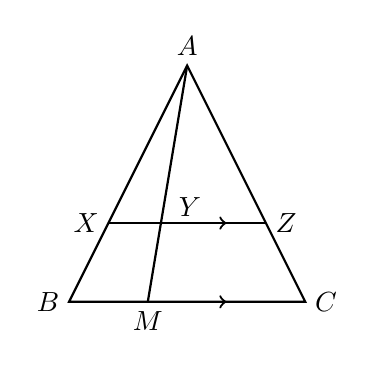
\begin{tikzpicture}

			\coordinate [label=left:$B$] (B) at (0,0);
			\coordinate [label=right:$C$] (C) at (3,0);
			\coordinate [label=above:$A$] (A) at (1.5,3);
			\draw [thick] [->] (0,0)--(2,0);
			\draw [thick] (B)--(C)--(A)--cycle;

			\coordinate [label=left:$X$] (X) at (0.5,1);
			\coordinate [label=left:$Y$] (Y) at (1.8,1.2);
			\coordinate [label=right:$Z$] (Z) at (2.5,1);
			\draw [thick] [->] (1,1)--(2,1);
			\draw [thick] (X)--(Z);

			\coordinate[label=below:$M$] (M) at (1,0);
			\draw [thick] [-] (1.5,3)--(1,0);
		\end{tikzpicture}
		\end{center}

	\item In the given figure, $DE$ $||$ $BC$. If $AD$ = 2units, $DB$ = $AE$ = 3units and $EC$ = $x$units, then find the value of $x$ is:
		\begin{center}
			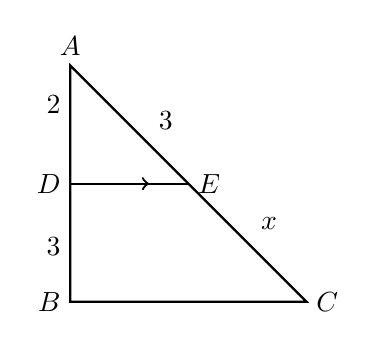
\begin{tikzpicture}
				\coordinate [label=left:$B$] (B) at (0,0);
				\coordinate [label=right:$C$] (C) at (3,0);
				\coordinate [label=above:$A$] (A) at (0,3);
				\draw [thick] (B)--(C)--(A)--cycle;

				\coordinate [label=left:$D$] (D) at (0,1.5);
				\coordinate [label=right:$E$] (E) at (1.5,1.5);
				\draw [thick] [->] (0,1.5)--(1,1.5);
				\draw [thick] (D)--(E);

				\coordinate [label=left:$3$] (3) at (0,0.7);
				\coordinate [label=left:$2$] (2) at (0,2.5);
				\coordinate [label=right:$3$] (3) at (1,2.3);
				\coordinate [label=right:$x$] (x) at (2.3,1);

			\end{tikzpicture}
		\end{center}

			\begin{enumerate}
				\item 2
				\item 3
				\item 5
				\item $\frac{9}{2}$
			\end{enumerate}

		\newpage

	\item In the given figure, $\Delta ABC$ and $\Delta DBC$ are on te same base $BC$. If $AD$ intersects $BC$ at O, prove that $\frac { ar(\Delta ABC)}{ar (\Delta DBC)}$ = $\frac{AO}{DO}$.

		\begin{center}
			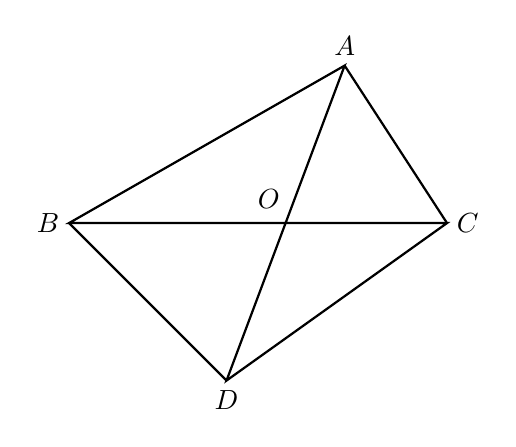
\begin{tikzpicture}
				\coordinate [label=below:$D$] (D) at (0,0);
				\coordinate [label=left:$B$] (B) at (-2,2);
				\coordinate [label=right:$C$] (C) at (2.8,2.);
				\coordinate [label=above:$A$] (A) at (1.5,4);
				\draw [thick] (A)--(B)--(C)--(D)--cycle;
				\draw [thick] (A)--(C);
				\draw [thick] (B)--(D);

				\coordinate [label=left:$O$] (O) at (0.8,2.3);

			\end{tikzpicture}
		\end{center}

\pagebreak

\title{\textbf{Linear}}
\date{}
\maketitle

	\item \textbf{Assertion (A):} Point $\vec{P}$(0,2) is the point of intersection of $y-axis$ with  the line $3x+2y=4$.\\
		\textbf{Reason (R):} The distance of point $\vec{P}$(0,2) from $x-axis$ is 2 units.


	\item If the pair of equations $3x-y+8=0$ and $6x-ry+16=0$ represent coincident lines, then the value of \text{'$r$'} is:

		\begin{enumerate}
			\item $-\frac{1}{2}$
			\item $\frac{1}{2}$
			\item -2
			\item 2
		\end{enumerate}

	\item The of linear equations $2x=5y+6$ and $15y=6x-18$ represents two lines which are:

			\begin{enumerate}
				\item intersecting
				\item parallel
				\item coincident
				\item either intersecting or parallel
			\end{enumerate}

		\item Find the equations of the diagonals of the parallelogram $\vec{PQRS}$ whose vertices are $\vec{P}$(4,2,-6), $\vec{Q}$(5,-3,1), $\vec{R}$(12,4,5) and $\vec{S}$(11,9,-2). Use these equations to find the point of intersection of diagonals.

	\item A line $l$ passes through point (-1,3,-2) and is perpendicular to both the lines $\frac {x}{1}=\frac{y}{2}=\frac{z}{3}$ and $\frac {x+2}{-3}=\frac{y-1}{2}=\frac{z+1}{5}$. Find the ctor equation of the line $l$. Hence, obtain its distance from origin.

\end{enumerate}
\end{document}
